Tämä kappale tulee luultavasti muuttumaan, yleisiä juttuja johdantoon ja tähän vain Oauth-spesifistä asiaa, miten eroaa kerberoksesta jne. Pituus 2-3 sivua, kuvia yms. Oleellisin näistä protokollista, koska tullaan käyttämään toteutuksessa.

OAuth on avoin tunnistautumisrajapinta hajautetuille web-sovelluksille. Se mahdollistaa käyttäjien resurssien jakamisen palveluiden välillä ilman käyttäjätunnuksen tai salasanan luovuttamista kolmannelle osapuolelle. Se perustuu erilaisten valtuutusavainten (token) välittämiseen palveluiden välillä. OAuth on yleisesti käytössä web-sovelluksissa, joissa halutaan näyttää käyttäjälle kuuluvia resursseja (esimerkiksi valokuvia), jotka sijaitsevat toisessa sovelluksessa [TODO: lähde].

OAuth on määritelty RFC-dokumentissa numero 5849. Sen ensimmäinen versio (1.0) julkaistiin lokakuussa 2007 ja päivitetty versio (1.0a) kesäkuussa 2009 \cite{oauth2_0}. OAuthin versio 2.0 on myös kehitteillä ja se on tarkoitus julkaista marraskuussa 2012 \cite{oauth2_0}.

Alunperin OAuthin kehitystyö alkoi marraskuussa 2006, kun Blaine Cook kehitty Twitter-palveluun OpenID-tukea.

... tarvitaanko tätä?

\begin{figure}[ht]
\centering
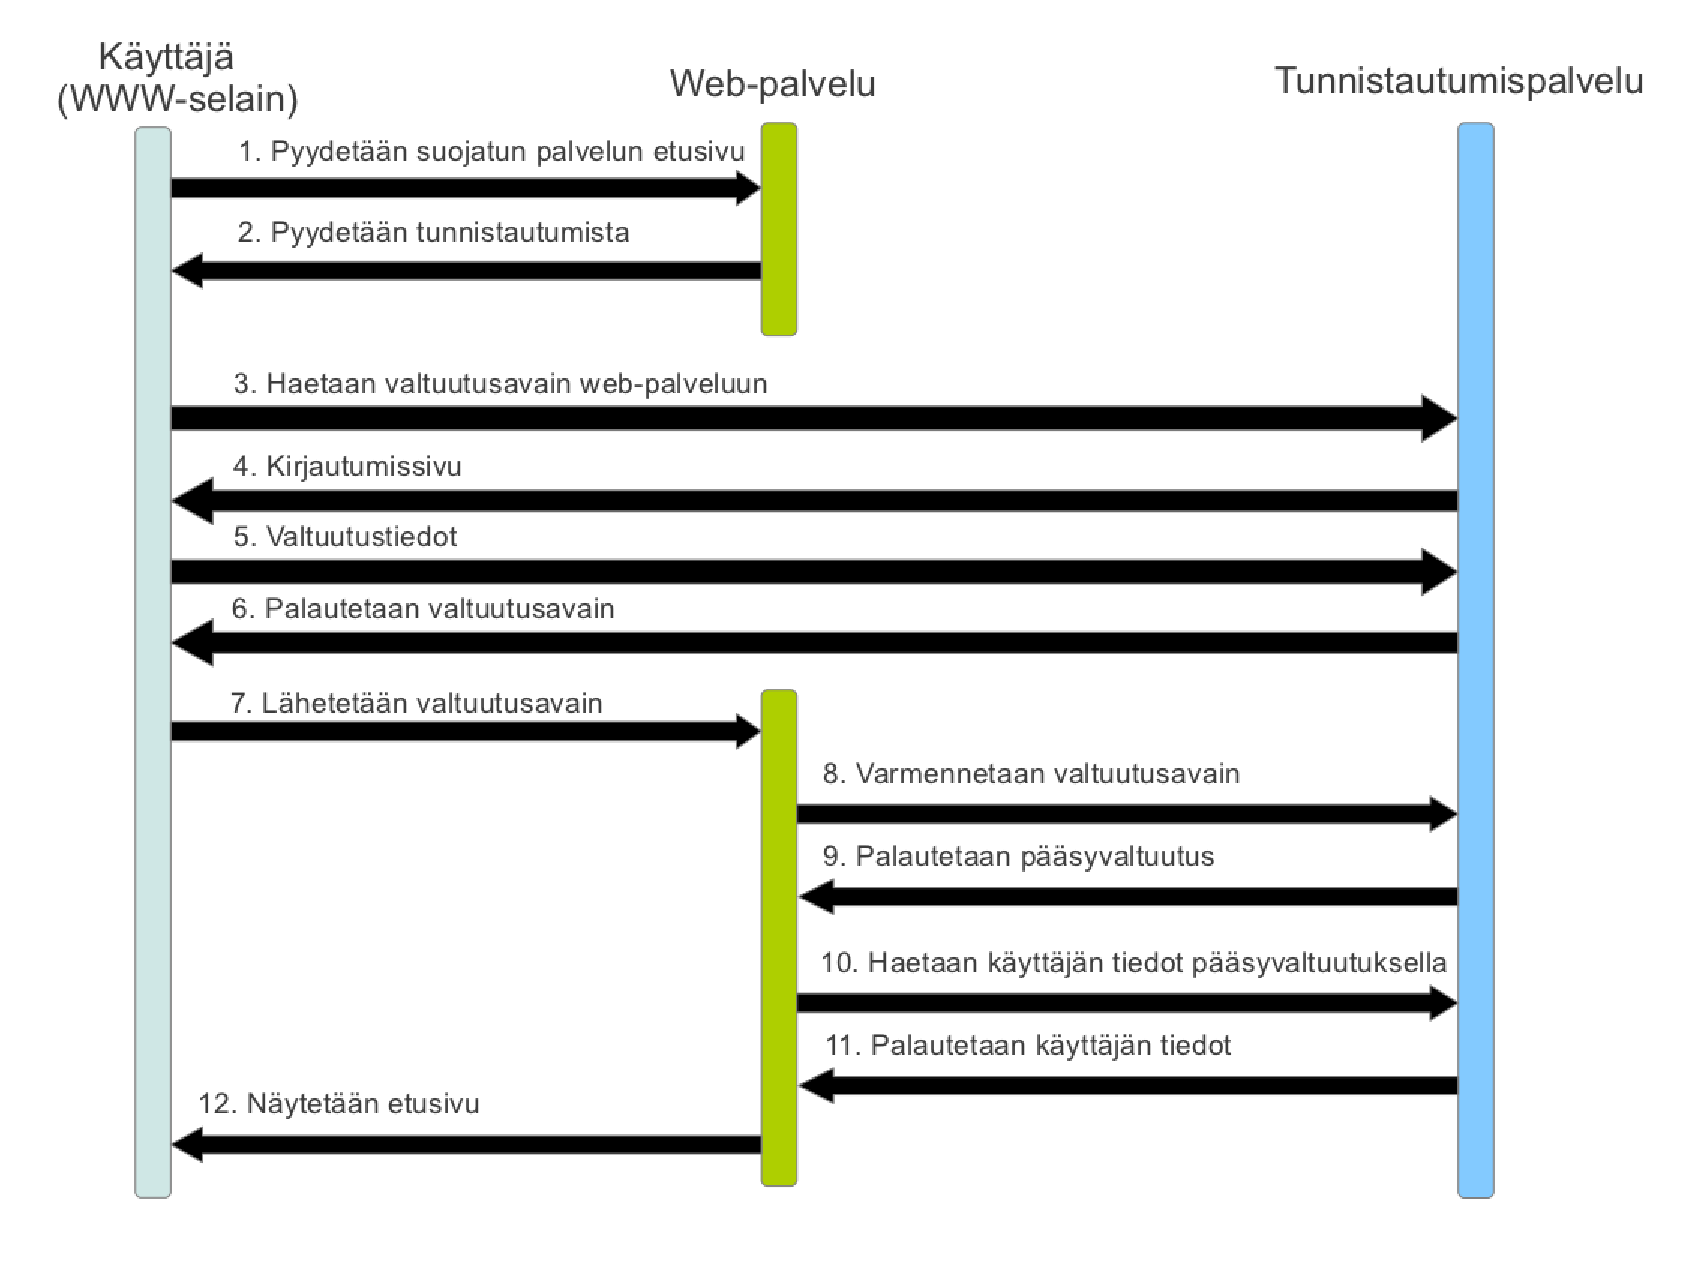
\includegraphics[width=\textwidth]{teknologiat/protokollat/oauth.eps}
\caption{OAuth sekvenssikaavio}%
\label{oauth}
\end{figure}
